% !TeX root = ../main.tex
% Add the above to each chapter to make compiling the PDF easier in some editors.

\chapter{Building Flows in Weight-Space}\label{chapter:method}

{\color{TUMBlue}
All the background discussion comes together here. Explain everything, referring to earlier work and connecting them with the other relevant topics. 
}

\section{Collecting Data}

\section{Flows with Geometries}

\subsection{Euclidean Flow}

\subsection{Normalized Flow}

\subsection{Geometric Flow}

{\color{TUMBlue} Mention how this can be extended to different geometries}

\section{Model}

\section{Training}

\begin{itemize}
    \item Predicting the target 
    \item couplings? 
    \item Sampling time
    \item Maybe some notes on how to train a flow model? Add to the review or maybe mention references here. Also do some reading. 
\end{itemize}

\section{Sampling}

\subsection{Deterministic Sampling}

\subsection{Stochastic Sampling }

\subsection{Guidance}

\begin{figure}[h!]
    \centering
    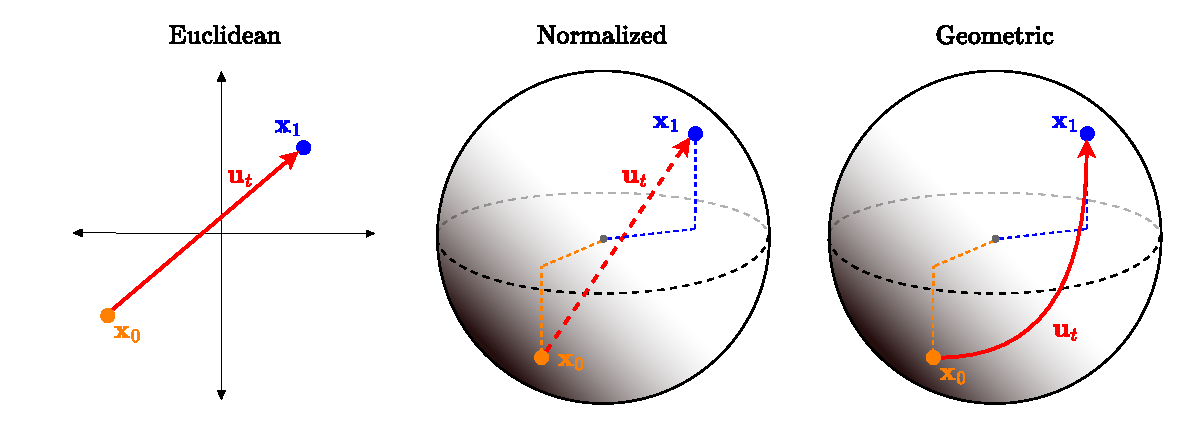
\includegraphics[width=\textwidth]{figures/flow_types.drawio.pdf}
    \caption{\label{fig:flow_types} Flow Types}
\end{figure}

\begin{figure}[h!]
    \centering
    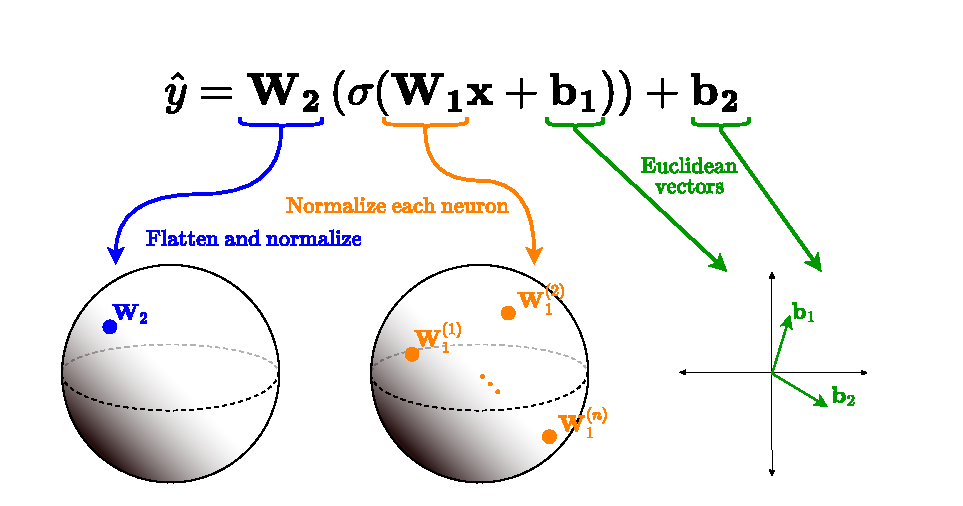
\includegraphics[width=\textwidth]{figures/canonicalization.drawio.pdf}
    \caption{\label{fig:canonicalization} Canonicalization}
\end{figure}